%%%%%%%%%%%%%%%%%%%%%%%%%%%%%%%%%%%%%%%%%
% Beamer Presentation
% LaTeX Template
% Version 1.0 (10/11/12)
%
% This template has been downloaded from:
% http://www.LaTeXTemplates.com
%
% License:
% CC BY-NC-SA 3.0 (http://creativecommons.org/licenses/by-nc-sa/3.0/)
%
%%%%%%%%%%%%%%%%%%%%%%%%%%%%%%%%%%%%%%%%%

%----------------------------------------------------------------------------------------
%	PACKAGES AND THEMES
%----------------------------------------------------------------------------------------
\documentclass[aspectratio=169]{beamer}
\usepackage[portuges]{babel}
\usepackage[utf8]{inputenc}
\usepackage[alf]{abntex2cite}	
\usepackage[portuguese, linesnumbered, vlined, titlenumbered, ruled]{algorithm2e}
\SetKwRepeat{Registro}{registro \{}{\}}%
\usepackage{beamerthemesplit}
\usepackage{multirow}
\usepackage{scalefnt}

% The Beamer class comes with a number of default slide themes
% which change the colors and layouts of slides. Below this is a list
% of all the themes, uncomment each in turn to see what they look like.

%\usetheme{default}
%\usetheme{AnnArbor}
%\usetheme{Antibes}
%\usetheme{Bergen}
%\usetheme{Berkeley}
%\usetheme{Berlin}
%\usetheme{Boadilla}
%\usetheme{CambridgeUS}
%\usetheme{Copenhagen}
%\usetheme{Darmstadt}
%\usetheme{Dresden}
%\usetheme{Frankfurt}
%\usetheme{Goettingen}
%\usetheme{Hannover}
%\usetheme{Ilmenau}
%\usetheme{JuanLesPins}
%\usetheme{Luebeck}
\usetheme{Madrid}
%\usetheme{Malmoe}
%\usetheme{Marburg}
%\usetheme{Montpellier}
%\usetheme{PaloAlto}
%\usetheme{Pittsburgh}
%\usetheme{Rochester}
%\usetheme{Singapore}
%\usetheme{Szeged}
%\usetheme{Warsaw}

% As well as themes, the Beamer class has a number of color themes
% for any slide theme. Uncomment each of these in turn to see how it
% changes the colors of your current slide theme.

%\usecolortheme{albatross}
%\usecolortheme{beaver}
%\usecolortheme{beetle}
%\usecolortheme{crane}
\usecolortheme{dolphin}
%\usecolortheme{dove}
%\usecolortheme{fly}
%\usecolortheme{lily}
%\usecolortheme{orchid}
%\usecolortheme{rose}
%\usecolortheme{seagull}
%\usecolortheme{seahorse}
%\usecolortheme{whale}
%\usecolortheme{wolverine}

%\setbeamertemplate{footline} % To remove the footer line in all slides uncomment this line
%\setbeamertemplate{footline}[page number] % To replace the footer line in all slides with a simple slide count uncomment this line

%\setbeamertemplate{navigation symbols}{} % To remove the navigation symbols from the bottom of all slides uncomment this line


\usepackage{graphicx} % Allows including images
\usepackage{booktabs} % Allows the use of \toprule, \midrule and \bottomrule in tables

%----------------------------------------------------------------------------------------
%	TITLE PAGE
%----------------------------------------------------------------------------------------
%%%%%%%%%%%%%%%%%%%%%%%%%%%%%%%%%%%%%%%%%%%%%%%%%%%%%%%%%%%%%%%%%%%%%%%%%%%%%%%%%%%%%%%%%
\title[Pilha, Fila e Lista]{Algoritmos e Estrutura de Dados II}
\subtitle{Pilha, Fila e Lista\\(Alocação Dinâmica)}
\author[Frederico Santos de Oliveira]{prof. Frederico Santos de Oliveira}
\institute[UFMT]{Universidade Federal de Mato Grosso\\ Instituto de Engenharia}
\date{}

\begin{document}

%------------------------------------------------
\begin{frame}
\titlepage % Print the title page as the first slide

\begin{figure}[!h]
  \centering
   
\includegraphics[width=80pt]{imgs/introducao.png}
  \label{fig_introducao}
\end{figure}
\end{frame}

%------------------------------------------------

\begin{frame}
\frametitle{Roteiro} % Table of contents slide, comment this block out to remove it
\tableofcontents % Throughout your presentation, if you choose to use \section{} and \subsection{} commands, these will automatically be printed on this slide as an overview of your presentation
\end{frame}

%----------------------------------------------------------------------------------------
%	PRESENTATION SLIDES
%----------------------------------------------------------------------------------------

%------------------------------------------------
\section{Objetivos}

\begin{frame}
\frametitle{Objetivos}

Esta aula tem como objetivos:

\begin{enumerate}
\item Apresentar os conceitos básicos sobre filas, pilhas e listas;
\item Explicitar as diferenças, vantagens e desvantagens de cada um;
\item Exemplificar os algoritmos por meio de pseudo-códigos.
\end{enumerate}

\end{frame}

%------------------------------------------------
% 
% \section{Referências bibliográficas}
%   \frame{\frametitle{Referências bibliográficas}
%     \bibliographystyle{abntex2-alf}
%     \bibliography{referencias}
%   }
%   
%------------------------------------------------
\section{Introdução} % Sections can be created in order to organize your presentation into discrete blocks, all sections and subsections are automatically printed in the table of contents as an overview of the talk
%------------------------------------------------

\begin{frame}
\frametitle{Introdução}
\begin{itemize}
 \item Alocação Dinâmica é o processo de solicitar e utilizar memória durante a execução de um programa. 
 \item Ela é utilizada para que um programa em C utilize apenas a memória necessária pra sua execução, sem desperdícios de memória. 
 \item Um exemplo de desperdício de memória é quando um vetor de 1000 posições é declarado quando não se sabe, de fato, se as 1000 posiçoes serão necessárias.
 \item A alocação dinâmica de memória deve ser utilizada quando não se sabe quanto espaço de memória será necessário pra o armazenamento de algum ou alguns valores. 
\end{itemize}
\end{frame}

\begin{frame}
\frametitle{Vantagens e Desvantagens}
\begin{itemize}
 \item Vantagens
 \begin{itemize}
 \item Ocupa espaço estritamente necessário
 \end{itemize}
 \item Desvantagens
 \begin{itemize}
 \item Custos usuais da alocação dinâmica (tempo de alocação, campos de ligação)
 \end{itemize} 
\end{itemize}
\end{frame}
%------------------------------------------------

\section{Estrutura Nodo}

\begin{frame}
\frametitle{Estrutura Nodo}
\begin{itemize}
 \item A  entidade elementar de uma estrutura de dados é o {\bf nodo} (pronuncia-se nó). 
 \item Um nodo é diferenciado pelo seu endereço relativo dentro da estrutura  e pode ser constituído de um ou vários campos. 
 \item Cada campo de um nodo armazena uma informação, um dado, que pode ser do tipo numérico, alfanumérico, lógicos, imagens, sons, enfim, qualquer informação que possa ser manipulada. 
 \item Todos os nodos de uma mesma estrutura devem ter a mesma configuração. 
\end{itemize}
\end{frame}


\begin{frame}
\frametitle{Estrutura Nodo}
Cada nodo armazena:
\begin{itemize}
 \item Um elemento.
  \begin{itemize}
  \item pode ser um inteiro, uma string, um vetor, um registro, não importa. 
  \item Aqui é denominado apenas {\bf item}.
  \end{itemize}  
 \item Uma ligação para o próximo nodo. 
 \begin{itemize}
 \item Em termos de implementação, trata-se de um ponteiro do tipo nodo, o qual denominaremos {\bf prox}.
 \end{itemize}
 \end{itemize}
\begin{figure}[!h]
  \centering
   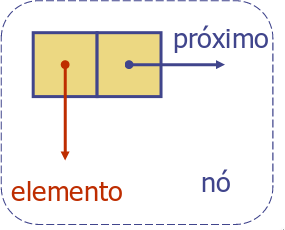
\includegraphics[width=100pt]{imgs/nodo.png}
  \label{fig_introducao}
\end{figure}
\end{frame}


\begin{frame}[fragile]{Estrutura Nodo}
\begin{algorithm}[H]
\caption{Nodo} 
\label{Nodo}
\Inicio{
 \Registro{Nodo}{
    Inteiro: item; \\
    Ponteiro Nodo: prox; 
  }
}
\end{algorithm} 
\end{frame}

%------------------------------------------------
\section{Pilhas}
%------------------------------------------------

\begin{frame}
\frametitle{Implementação Dinâmica}
\framesubtitle{Pilhas}
\centering
\huge{Implementação Dinâmica\\
Pilhas
}
\end{frame}

\begin{frame}
\frametitle{Estrutura Pilha}
A seguir, são apresentadas as caracteristicas da estrutura de dados Pilha:
\begin{itemize}
 \item Existem dois ponteiros:
 \begin{itemize}
    \item um aponta para o {\bf topo} da Pilha.
    \item o outro que aponta para o {\bf fundo} da Pilha.
 \end{itemize}
 \item No topo da Pilha existe um nodo vazio (denominado nodo {\bf cabeça}).
 \item O ponteiro topo sempre aponta para o nodo cabeça.
 \item Quando a Pilha está vazia, fundo e topo apontam para o nodo cabeça.
\end{itemize}
\end{frame}

\begin{frame}[fragile]{Estrutura Pilha}
\begin{algorithm}[H]
\caption{Pilha} 
\label{Pilha}
\Inicio{
 \Registro{Pilha}{
    Ponteiro Nodo: topo, fundo; 
  }
}
\end{algorithm} 
\end{frame}

%------------------------------------------------
% 
% \begin{frame}{Estrutura Pilha}{Pilha nao-Vazia}
% \begin{figure}[!h]
%   \centering
%   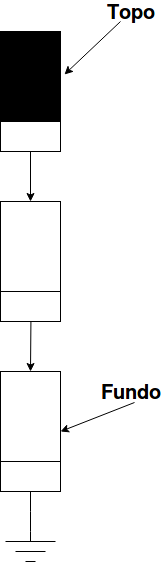
\includegraphics[width=50pt]{imgs/pilha_nao_vazia.png}
%   \label{fig_pilha_nao_vazia}
% \end{figure}
% \end{frame}

%------------------------------------------------
% 
% \begin{frame}{Estrutura Pilha}{Pilha Vazia}
% \begin{figure}[!h]
%   \centering
%   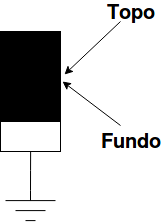
\includegraphics[width=50pt]{imgs/pilha_vazia.png}
%   \label{fig_pilha_vazia}
% \end{figure}
% \end{frame}

%------------------------------------------------

\begin{frame}
\frametitle{Pilhas - Operações básicas}
\begin{enumerate}
 \item CriaPilhaVazia($S$) 
 \item boolean PilhaVazia($S$)
 \item Empilha($S$,$x$)
 \item int Desempilha($S$) 
 \item ApagaPilha($S$);
\end{enumerate}
\end{frame}

%------------------------------------------------

\begin{frame}
\frametitle{Pilha - Implementação com ponteiros}
% \scalebox{0.5}{
\begin{algorithm}[H]
\caption{CriaPilhaVazia} 
\label{CriaPilhaVazia}
\Entrada{Pilha S.}
\Inicio{
  S.topo $\leftarrow$ ALOCA\_NODO()\\
  S.fundo $\leftarrow$ S.topo\\
  S.topo.prox $\leftarrow$  NULL \\
%   $S.tamanho \leftarrow 0$ 
}
\end{algorithm}
\end{frame}

%------------------------------------------------

\begin{frame}
\frametitle{Pilhas - Implementação com ponteiros}
% \scalebox{0.5}{
\begin{algorithm}[H]
\caption{PilhaVazia} 
\label{PilhaVazia}
\Entrada{Pilha S.}
\Saida{Booleano (V ou F) indicando se S está vazia.}
\Inicio{
  \Se { (S.topo = S.fundo) } {
    \Retorna Verdadeiro \\
    }
  \Senao {
    \Retorna Falso
  } 
}
\end{algorithm}
% }  
\end{frame}

%------------------------------------------------
% 
% \begin{frame}{Pilhas - Implementação com ponteiros}{Operaçao Empilha}
% \begin{figure}[!h]
%   \centering
%   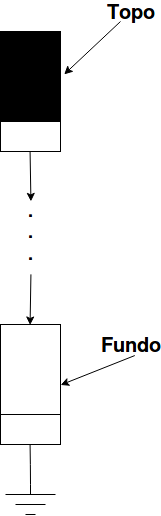
\includegraphics[width=40pt]{imgs/empilhar_passo0.png}
%   \label{fig_empilhar_passo0}
% \end{figure}
% \end{frame}

%------------------------------------------------
% 
% \begin{frame}[fragile]{Pilhas - Implementação com ponteiros}{Empilha - Passo-a-Passo}
% \begin{figure}[!h]
%   \centering
%   passo 1
%   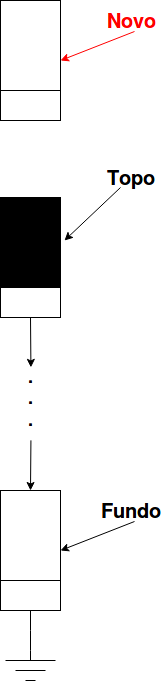
\includegraphics[width=40pt]{imgs/empilhar_passo1.png}
%   Passo 2
%   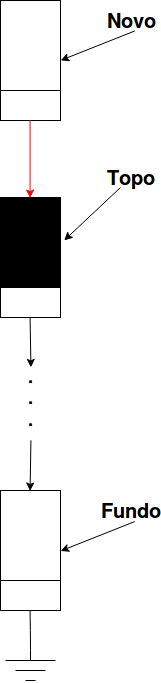
\includegraphics[width=40pt]{imgs/empilhar_passo2.png}
%   Passo 3
%   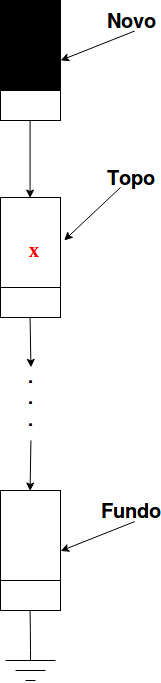
\includegraphics[width=40pt]{imgs/empilhar_passo3.png}
%   Passo 4
%   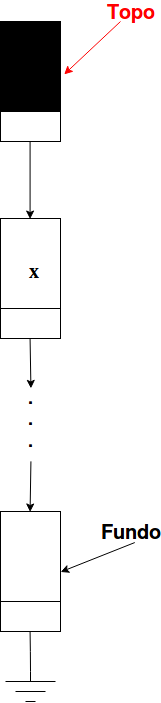
\includegraphics[width=40pt]{imgs/empilhar_passo4.png}  
%   \label{fig_empilhar_passo1}
% \end{figure}
% \end{frame}

%------------------------------------------------


\begin{frame}
\frametitle{Pilhas - Implementação com ponteiros}
% \scalebox{0.5}{
\begin{algorithm}[H]
\caption{Empilha} 
\label{Empilha}
\Entrada{Pilha S, item x.}
\Inicio{
  novo $\leftarrow$ ALOCA\_NODO() \\
  novo.prox $\leftarrow$ S.topo \\
  S.topo.item $\leftarrow$ x \\  
  S.topo $\leftarrow$ novo \\
%   $p.tamanho \leftarrow p.tamanho + 1$
}
\end{algorithm}
% }  
\end{frame}

%------------------------------------------------

\begin{frame}
\frametitle{Pilhas - Implementação com ponteiros}
% \scalebox{0.5}{
\begin{algorithm}[H]
\caption{Desempilha} 
\label{Desempilha}
\Entrada{Pilha S.}
\Saida{Item desempilhado.}
\Inicio{
  \Se {(PilhaVazia(S))}  
  { 
    Imprima "Erro {\it underflow}: pilha vazia." \\ 
  }
  \Senao {
    aux $\leftarrow$ S.topo \\
    S.topo $\leftarrow$ aux.prox \\
    item $\leftarrow$ aux.prox.item \\
    DESALOCA\_NODO(aux)\\  
    \Retorna item
  }
%   $S.tamanho \leftarrow S.tamanho - 1$ 
}
\end{algorithm}
% }  
\end{frame}

%------------------------------------------------

\begin{frame}
\frametitle{Pilha - Implementação com ponteiros}
% \scalebox{0.5}{
\begin{algorithm}[H]
\caption{ApagaPilha} 
\label{ApagaPilha}
\Entrada{Pilha S.}
\Inicio{
  \Enqto {(NOT(PilhaVazia(S)))} {
    \CommentSty{// Ignora o elemento desempilhado.}\\
    Desempilha(S)\\
  }
  \CommentSty{// Apaga o nodo cabeça.}\\
  DESALOCA\_NODO(S.topo)\\
  S.topo $\leftarrow$ NULL \\
  S.fundo $\leftarrow$ NULL \\
%   $S.tamanho \leftarrow 0$ 
}
\end{algorithm}
\end{frame}


%------------------------------------------------
\section{Filas}
%------------------------------------------------

\begin{frame}
\frametitle{Implementação Dinâmica}
\framesubtitle{Filas}
\centering
\huge{Implementação Dinâmica\\
Filas
}
\end{frame}

\begin{frame}
\frametitle{Estrutura Fila}
A seguir, são apresentadas as caracteristicas da estrutura de dados Fila:
\begin{itemize}
 \item Existem dois ponteiros:
 \begin{itemize}
    \item um aponta para o {\bf início} da Fila.
    \item o outro que aponta para o {\bf fim} da Fila.
 \end{itemize}
 \item No início da Fila existe um nodo vazio (denominado nodo {\bf cabeça}).
 \item O ponteiro início sempre aponta para o nodo cabeça.
 \item Quando a Fila está vazia, início e fim apontam para o nodo cabeça.
\end{itemize}
\end{frame}


\begin{frame}[fragile]{Estrutura Fila}
\begin{algorithm}[H]
\caption{Fila} 
\label{Fila}
\Inicio{
 \Registro{Fila}{
    Ponteiro Nodo: início, fim; 
  }
}
\end{algorithm} 
\end{frame}


\begin{frame}
\frametitle{Filas - Operações básicas}
\begin{enumerate}
 \item CriaFilaVazia($Q$) 
 \item boolean FilaVazia($Q$)
 \item Enfileira($Q$,$x$)
 \item int Desenfileira($Q$) 
 \item ApagaFila($Q$)
\end{enumerate}
\end{frame}

%------------------------------------------------

\begin{frame}
\frametitle{Filas - Implementação com ponteiros}
% \scalebox{0.5}{
\begin{algorithm}[H]
\caption{CriaFilaVazia} 
\label{CriaFilaVazia}
\Entrada{Fila Q.}
\Inicio{
  Q.inicio $\leftarrow$ ALOCA\_NODO() \\
  Q.fim $\leftarrow$ Q.inicio \\
  Q.inicio.prox $\leftarrow$ NULL
}
\end{algorithm}
% }  
\end{frame}

%------------------------------------------------

\begin{frame}
\frametitle{Filas - Implementação com ponteiros}
% \scalebox{0.5}{
\begin{algorithm}[H]
\caption{FilaVazia} 
\label{FilaVazia}
\Entrada{Fila Q.}
\Saida{Booleano (V ou F) indicando se Q está vazia.}
\Inicio{
  \Se {(Q.inicio = Q.fim)} {
  	\Retorna VERDADEIRO\\
  }
  \Senao{
    	\Retorna FALSO\\
  }
}
\end{algorithm}
% }  
\end{frame}

%------------------------------------------------

\begin{frame}
\frametitle{Filas - Implementação com ponteiros}
% \scalebox{0.5}{
\begin{algorithm}[H]
\caption{Enfileira} 
\label{Enfileira}
\Entrada{Fila Q, item x.}
\Inicio{
  Q.fim.prox $\leftarrow$ ALOCA\_NODO() \\
  Q.fim $\leftarrow$ Q.fim.prox \\
  Q.fim.item $\leftarrow$ x \\
  Q.fim.prox $\leftarrow$ NULL 
}
\end{algorithm}
% }  
\end{frame}


%------------------------------------------------

\begin{frame}
\frametitle{Filas - Implementação com ponteiros}
% \scalebox{0.5}{
\begin{algorithm}[H]
\caption{Desenfileira} 
\label{Desenfileira}
\Entrada{Fila Q.}
\Saida{Item desenfileirado.}
\Inicio{
  \Se { ( FilaVazia(Q) ) } { 
    Imprima "Erro {\it underflow}: fila esta vazia." \\  
  }
  \Senao {
    aux $\leftarrow$ Q.inicio \\
    Q.inicio $\leftarrow$ Q.inicio.prox \\
    item $\leftarrow$ Q.inicio.item \\
    aux.prox $\leftarrow$ NULL\\
    DESALOCA\_NODO(aux) \\
    \Retorna item
  }
}
\end{algorithm}
% }  
\end{frame}

%------------------------------------------------

\begin{frame}
\frametitle{Filas - Implementação com ponteiros}
% \scalebox{0.5}{
\begin{algorithm}[H]
\caption{ApagaFila} 
\label{ApagaFila}
\Entrada{Fila Q.}
\Inicio{
  \Enqto {(NOT(FilaVazia(Q)))} {
    \CommentSty{// Ignora o elemento desenfileirado.}\\
    Desenfila(Q)\\
  }
  \CommentSty{// Apaga o nodo cabeça.}\\
  DESALOCA\_NODO(Q.inicio)\\
  Q.inicio $\leftarrow$ NULL \\
  Q.fim $\leftarrow$ NULL \\
%   $S.tamanho \leftarrow 0$ 
}
\end{algorithm}
\end{frame}
%------------------------------------------------
\section{Listas}
%------------------------------------------------


\begin{frame}{Implementação Dinâmica}{Listas}
\centering
\huge{Implementação Dinâmica\\
Listas
}
\end{frame}


\begin{frame}
\frametitle{Listas}
A estrutura e funcionamento de uma lista encadeada é semelhante a dos vetores, porém, com algumas diferenças importantes:
\begin{itemize}
 \item Os elementos dos vetores podem ser acessados diretamente. Nas listas, os nós são acessados sequencialmente, pelos ponteiros;
 \item O espaço previsto para vetores já é alocado e fica reservado. Nas listas, o espaço de memória é alocada conforme necessário.
\end{itemize}
\end{frame}

\subsection{Lista Simplesmente Encadeada}

\begin{frame}
\frametitle{Estrutura Lista}
A seguir, são apresentadas as caracteristicas da estrutura de dados Lista:
\begin{itemize}
 \item Existem dois ponteiros:
 \begin{itemize}
    \item um aponta para o {\bf primeiro} nodo da Lista.
    \item o outro que aponta para o {\bf último} nodo da Lista.
 \end{itemize}
 \item Diferentemente da Pilha e da Fila, \underline{não existe} o nodo {\bf cabeça}.
 \item Quando a Lista está vazia, os ponteiros primeiro e último apontam para NULL.
\end{itemize}
\end{frame}


\begin{frame}[fragile]{Estrutura Lista}
\begin{algorithm}[H]
\caption{Lista} 
\label{Lista}
\Inicio{
 \Registro{Lista}{
    Ponteiro Nodo: primeiro, último; 
  }
}
\end{algorithm} 
\end{frame}

%------------------------------------------------

\begin{frame}[fragile]{Estrutura Nodo}
\begin{algorithm}[H]
\caption{Nodo} 
\label{Nodo}
\Inicio{
 \Registro{Nodo}{
    Inteiro: item; \\
    Ponteiro Nodo: prox; 
  }
}
\end{algorithm} 
\end{frame}

%------------------------------------------------

\begin{frame}
\frametitle{Listas}
Tipos de Listas
\begin{itemize}
 \item Simplesmente encadeada; 
 \item Duplamente encadeada;
 \item Circular.
\end{itemize}
\end{frame}

%------------------------------------------------

\begin{frame}{Lista Simplesmente Encadeada}
\begin{figure}[!h]
  \centering
  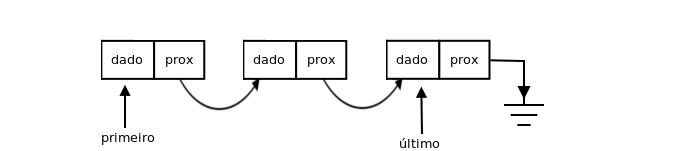
\includegraphics[width=300pt]{imgs/lista_simplesmente_encadeada.png}
  \label{fig_lista_encadeada}
\end{figure}
\end{frame}

%------------------------------------------------

\begin{frame}{Lista Simplesmente Encadeada}{Operações básicas}
\begin{enumerate}
 \item CriaListaVazia($L$)
 \item boolean ListaVazia($L$)
 \item int ListaBuscar($L$, $x$)
 \item int ListaBuscarPosição($L$, $p$)
 \item ListaInserirInício($L$, $x$)
 \item ListaInserirFinal($L$, $x$)
 \item ListaInserirPosição($L$, $x$, $p$)
 \item ApagarLista($L$)
 \item int ListaRemoverInício($L$) 
 \item int ListaRemoverFinal($L$) 
 \item int ListaRemoverPosição($L$, $p$) 
\end{enumerate}
\end{frame}

%------------------------------------------------

\begin{frame}{Lista Simplesmente Encadeada}{Operações básicas}
% \scalebox{0.5}{
\begin{algorithm}[H]
\caption{CriaListaVazia} 
\label{CriaListaVazia}
\Entrada{Lista L.}
\Inicio{
  L.primeiro $\leftarrow$ NULL \\
  L.último $\leftarrow$ NULL \\
}
\end{algorithm}
% }  
\end{frame}


%------------------------------------------------

\begin{frame}{Lista Simplesmente Encadeada}{Operações básicas}
% \scalebox{0.5}{
\begin{algorithm}[H]
\caption{ListaVazia} 
\label{ListaVazia}
\Entrada{Lista L.}
\Saida{Booleano (V ou F) indicando se L está vazia.}
\Inicio{
  \Se {(L.primeiro = NULL)} {
    \Retorna Verdadeiro
  }
  \Senao {
    \Retorna Falso
  }
}
\end{algorithm}
% }  
\end{frame}

%------------------------------------------------

\begin{frame}{Lista Simplesmente Encadeada}{Operações básicas}
% \scalebox{0.5}{
\begin{algorithm}[H]
\caption{ListaBuscar} 
\label{ListaSimplesBuscar}
\Entrada{Lista L, item $x$.}
\Saida{Nodo que contém $x$ ou NULL caso não encontrado.}
\Inicio{
  aux $\leftarrow$ L.primeiro \\
  \Enqto {(aux $\neq$ NULL) AND (aux.item $\neq$ x) } {
      aux $\leftarrow$ aux.prox \\
  }
  \Retorna aux
}
\end{algorithm}
% }  
\end{frame}


%------------------------------------------------

\begin{frame}{Lista Simplesmente Encadeada}{Operações básicas}
% \scalebox{0.5}{
\begin{algorithm}[H]
\caption{ListaBuscarPosição} 
\label{ListaSimplesBuscarPosicao}
\Entrada{Lista L, posição $p$.}
\Saida{Nodo que se encontra na posição $p$ ou NULL caso não encontrado.}
\Inicio{
  aux $\leftarrow$ L.primeiro \\
  c $\leftarrow$ 1 \\
  \Enqto {(aux $\neq$ NULL) AND (c $<$ p) } {
      aux $\leftarrow$ aux.prox \\
      c $\leftarrow$ c + 1
  }
  \Retorna aux
}
\end{algorithm}
% }  
\end{frame}

%------------------------------------------------

\begin{frame}{Lista Simplesmente Encadeada}{Operações básicas}
% \scalebox{0.5}{
\begin{algorithm}[H]
\caption{ListaInserirInício} 
\label{ListaSimplesInserirInicio}
\Entrada{Lista L, item $x$.}
\Inicio{
  novo $\leftarrow ALOCA\_NODO()$ \\
  novo.item $\leftarrow$ x \\
  novo.prox $\leftarrow$ L.primeiro \\
  L.primeiro $\leftarrow$ novo \\
  \CommentSty{// Verifica se a lista está vazia.} \\
  \Se {(L.último = NULL)} {
    L.último $\leftarrow$ L.primeiro \\
  }
}
\end{algorithm}
% }  
\end{frame}

%------------------------------------------------

\begin{frame}{Lista Simplesmente Encadeada}{Operações básicas}
% \scalebox{0.5}{
\begin{algorithm}[H]
\caption{ListaInserirFinal} 
\label{ListaSimplesInserirFinal}
\Entrada{Lista L, item $x$.}
\Inicio{
  novo $\leftarrow ALOCA\_NODO()$ \\
  novo.item $\leftarrow$ x \\
  novo.prox $\leftarrow$ NULL \\
  \CommentSty{// Verifica se a lista está vazia.} \\
  \Se {(L.primeiro = NULL)} {
    L.primeiro $\leftarrow$ novo \\
    L.último $\leftarrow$ L.primeiro \\
  }
  \Senao {
    L.último.prox $\leftarrow$ novo \\
    L.último $\leftarrow$ novo \\
  }
}
\end{algorithm}
% }  
\end{frame}

%------------------------------------------------

\begin{frame}{Lista Simplesmente Encadeada}{Operações básicas}
\begin{itemize}
 \item O algoritmo a seguir insere um nodo com item $x$ na posição $p$ da lista.
 \item Não verifica se existe um nodo na posição $p$, simplesmente considera que o nodo existe.
 \item A seguir, uma descrição dos passos do algoritmo:
 \begin{enumerate}
    \item Primeiramente, verifica se $p$ é a primeira posição.
    \begin{itemize}
      \item Caso sim, invoca a função ListaInserirInicio.
      \item Caso contrário, busca o nodo na posição $p-1$, ou seja, o nodo anterior a $p$.
    \end{itemize}       
    \item Em seguida, insere o novo nodo entre os nodos nas posições $p-1$ (denominado {\it anterior}) e $p$ (denominado {\it proximo}).
    \item Por fim, verifica se o nodo inserido na posição $p$ é o último nodo da lista. Caso sim, atualiza o ponteiro último.
 \end{enumerate}
\end{itemize} 
\end{frame}

%------------------------------------------------

\begin{frame}{Lista Simplesmente Encadeada}{Operações básicas}
\scalebox{0.6} {
\begin{algorithm}[H]
\caption{ListaInserirPosição} 
\label{ListaSimplesInserirPosicao}
\Entrada{Lista L, item $x$, posição $p$.}
\Inicio{
  \CommentSty{// Verifica se o nodo deve ser inserido no início. }\\
  \Se {($p = 1$)} {
    ListaInserirInício(L, x) \\
  }
  \Senao {
    novo $\leftarrow ALOCA\_NODO()$ \\
    novo.item $\leftarrow$ x \\  
    \CommentSty{// Busca o nodo na posição anterior a $p$.}\\
    anterior $\leftarrow$ ListaBuscarPosição(L,$p-1$) \\
    \CommentSty{// Insere o novo nodo entre os nodos} \\
    \CommentSty{// anterior e posterior.}\\
    posterior $\leftarrow$ anterior.prox \\
    anterior.prox $\leftarrow$ novo \\  
    novo.prox $\leftarrow$ posterior \\
    \CommentSty{// Verifica se o nodo na posição $p-1$ é o último,}\\
    \CommentSty{// ou seja, seu posterior é NULL.} \\
    \Se {(posterior = NULL)} {
      L.último $\leftarrow$ novo \\
    }   
  }
}
\end{algorithm}
}% scalebox  
\end{frame}

%------------------------------------------------

\begin{frame}{Lista Simplesmente Encadeada}{Operações básicas}
% \scalebox{0.5}{
\begin{algorithm}[H]
\caption{ApagarLista} 
\label{ApagarLista}
\Entrada{Lista L.}
\Inicio{
  aux $\leftarrow$ L.primeiro \\
  \Enqto {(L.primeiro $\neq$ NULL)} {
    L.primeiro $\leftarrow$ L.primeiro.prox \\
    DESALOCA\_NODO(aux) \\
    aux = L.primeiro 
  }
}
\end{algorithm}
% }  
\end{frame}

%------------------------------------------------

\begin{frame}{Lista Simplesmente Encadeada}{Operações básicas}
\scalebox{0.8}{
\begin{algorithm}[H]
\caption{ListaRemoverInício} 
\label{ListaSimplesRemoverInicio}
\Entrada{Lista L, item $x$.}
\Inicio{
  \CommentSty{// Verifica se a lista está vazia.} \\
  \Se {(ListaVazia(L))} {
      Imprima "Erro {\it underflow}: lista vazia" \\ 
  }
  \Senao {
    aux $\leftarrow$ L.primeiro \\    
    x $\leftarrow$ aux.item \\
    L.primeiro $\leftarrow$ L.primeiro.prox \\
    \CommentSty{// Verifica se a lista possui apenas um nodo.} \\
    \Se {(L.primeiro = NULL)} {
      \CommentSty{// Primeiro e Último apontam para NULL.} \\
      L.último $\leftarrow$ NULL \\
    }
    aux.prox $\leftarrow$ NULL \\
    DESALOCA\_NODO(aux) \\
    \Retorna x
  }
}
\end{algorithm}
}  
\end{frame}

%------------------------------------------------

\begin{frame}{Lista Simplesmente Encadeada}{Operações básicas}
\scalebox{0.5}{
\begin{algorithm}[H]
\caption{ListaRemoverFinal} 
\label{ListaSimplesRemoverFinal}
\Entrada{Lista L}
\Saida{Item removido}
\Inicio{
  \CommentSty{// Verifica se a lista está vazia.} \\
  \Se {(ListaVazia(L))} {
      Imprima "Erro {\it underflow}: lista vazia" \\ 
  }  
  \Senao {
    \CommentSty{// Verifica se a lista possui um único elemento.} \\  
    \Se{(L.primeiro = L.último) AND (NOT(ListaVazia(L)))} {
	aux $\leftarrow$ L.primeiro\\
	L.primeiro $\leftarrow$ NULL \\
	L.último $\leftarrow$ NULL \\
    }
    \CommentSty{// Caso contrário, a lista possui }\\
    \CommentSty{// pelo menos dois elementos.} \\  
    \Senao {
     \CommentSty{// Busca o penú	ltimo elemento.} \\  
      anterior $\leftarrow$ L.primeiro \\    
      \Enqto{(anterior.prox $\neq$ L.último)} {
	anterior $\leftarrow$ anterior.prox \\
      }
      aux $\leftarrow$ L.último \\
      anterior.prox $\leftarrow$ NULL \\
      L.último $\leftarrow$ anterior \\
    }
    x $\leftarrow$  aux.item \\
    aux.prox $\leftarrow$ NULL \\
    DESALOCA\_NODO(aux) \\  
    \Retorna x
  }
}
\end{algorithm}
}  
\end{frame}

%------------------------------------------------

\begin{frame}{Lista Simplesmente Encadeada}{Operações básicas}
\scalebox{0.56} {
\begin{algorithm}[H]
\caption{ListaRemoverPosição} 
\label{ListaSimplesRemoverPosicao}
\Entrada{Lista L, posição $p$}
\Saida{Item removido}
\Inicio{
  \CommentSty{// Verifica se a lista está vazia.} \\
  \Se {(ListaVazia(L))} {
      Imprima "Erro {\it underflow}: lista vazia" \\ 
  }
  \Senao {
    \CommentSty{// Verifica se o nodo a ser removido é o primeiro.}\\
    \Se {(p = 1)} {
      \Retorna ListaRemoverInicio(L) \\
    }
    \Senao {
      \CommentSty{// Busca o nodo na posição anterior a $p$.}\\
      anterior $\leftarrow$ ListaBuscarPosição(L,$p-1$) \\
      \CommentSty{// Remove o nodo na posição $p$, apontado por aux.}\\
      aux $\leftarrow$ anterior.prox \\
      posterior $\leftarrow$ aux.prox \\  
      anterior.prox $\leftarrow$ posterior \\
      \CommentSty{// Verifica se o nodo a ser removido é o último.}\\
      \Se {(aux = L.último)}  {
	L.último $\leftarrow$ anterior \\
      }   
      $x \leftarrow$ aux.item \\
      aux.prox $\leftarrow$ NULL \\
      DESALOCA\_NODO(aux) \\
      \Retorna $x$
    }
  }
}
\end{algorithm}
}% scalebox  
\end{frame}

\subsection{Lista Duplamente Encadeada}
%------------------------------------------------


\begin{frame}{Implementação Dinâmica}{Listas}
\centering
\huge{Implementação Dinâmica\\
Listas Duplamente Encadeadas
}
\end{frame}

%------------------------------------------------


\begin{frame}
\frametitle{Estrutura Lista}
A seguir, são apresentadas as características da Lista Duplamente Encadeada que são \underline{idênticas} à Lista Simplesmente Encadeada:
\begin{itemize}
 \item Existem dois ponteiros:
 \begin{itemize}
    \item um aponta para o {\bf primeiro} nodo da Lista.
    \item o outro que aponta para o {\bf último} nodo da Lista.
 \end{itemize}
 \item \underline{Não existe} o nodo {\bf cabeça}.
 \item Quando a Lista está vazia, os ponteiros primeiro e último apontam para NULL.
\end{itemize}
\end{frame}


\begin{frame}{Lista Duplamente Encadeada}{Estrutura Nodo}
Diferentemente do nodo presente na Lista Simplesmente Encadeada, na lista Duplamente Encadeada cada nodo armazena:
\begin{itemize}
 \item Um elemento.
  \begin{itemize}
  \item pode ser um inteiro, uma string, um vetor, um registro (não importa), também denominado {\bf item}.
  \end{itemize}  
 \item Uma ligação para o \underline{próximo} nodo.
 \item Uma ligação para o nodo \underline{anterior}.
 \end{itemize}
\end{frame}


\begin{frame}[fragile]{Lista Duplamente Encadeada}{Estrutura Nodo}
\begin{algorithm}[H]
\caption{Nodo} 
\label{Nodo}
\Inicio{
 \Registro{Nodo}{
    Inteiro: item; \\
    Ponteiro Nodo: prox, ant; 
  }
}
\end{algorithm} 
\end{frame}

%------------------------------------------------

\begin{frame}
\frametitle{Lista Duplamente Encadeada}
\begin{figure}[!h]
  \centering
  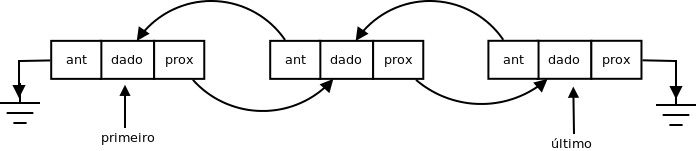
\includegraphics[width=300pt]{imgs/lista_duplamente_encadeada.png}
  \label{fig_lista_duplamente_encadeada}
\end{figure}
\end{frame}

%------------------------------------------------

\begin{frame}{Lista Duplamente Encadeada}{Operações básicas}
\begin{enumerate}
 \item ListaInserirInício($L$, $x$)
 \item ListaInserirFinal($L$, $x$)
 \item ListaInserirPosição($L$, $x$, $p$)
 \item int ListaRemoverInício($L$) 
 \item int ListaRemoverFinal($L$) 
 \item int ListaRemoverPosição($L$, $p$) 
\end{enumerate}
\end{frame}


%------------------------------------------------

\begin{frame}
\frametitle{Lista Duplamente Encadeada - Implementação}
% \scalebox{0.5}{
\begin{algorithm}[H]
\caption{ListaInserirInício} 
\label{ListaDuplaInserirInicio}
\Entrada{Lista $L$, item $x$.}
\Inicio{
  novo $\leftarrow$ ALOCA\_NODO() \\
  novo.item $\leftarrow$ x \\
  novo.prox $\leftarrow$ $L$.primeiro \\
  \CommentSty{// Verifica se a lista está vazia.} \\
  \Se {(ListaVazia(L))} {
    L.último $\leftarrow$ novo \\    
  }
  \Senao {
    L.primeiro.ant $\leftarrow$ novo \\
  }
  L.primeiro $\leftarrow$ novo \\
  L.primeiro.ant $\leftarrow$ NULL \\
}
\end{algorithm}
% }  
\end{frame}


%------------------------------------------------

\begin{frame}{Lista Duplamente Encadeada}{Operações básicas}
% \scalebox{0.5}{
\begin{algorithm}[H]
\caption{ListaInserirFinal} 
\label{ListaDuplaInserirFinal}
\Entrada{Lista L, item $x$.}
\Inicio{
  novo $\leftarrow ALOCA\_NODO()$ \\
  novo.item $\leftarrow$ x \\
  novo.prox $\leftarrow$ NULL \\
  \CommentSty{// Verifica se a lista está vazia.} \\
  \Se {(ListaVazia(L))} {
    L.primeiro $\leftarrow$ novo \\
  }
  \Senao {
    L.último.prox $\leftarrow$ novo \\
  }
  novo.ant $\leftarrow$ L.último \\
  L.último $\leftarrow$ novo \\  
}
\end{algorithm}
% }  
\end{frame}

%------------------------------------------------

\begin{frame}{Lista Duplamente Encadeada}{Operações básicas}
\scalebox{0.6} {
\begin{algorithm}[H]
\caption{ListaInserirPosição} 
\label{ListaDuplaInserirPosicao}
\Entrada{Lista L, item $x$, posição $p$.}
\Inicio{
  \CommentSty{// Verifica se o nodo deve ser inserido no início. }\\
  \Se {($p = 1$)} {
    ListaInserirInício(L, x) \\
  }
  \Senao {
    novo $\leftarrow ALOCA\_NODO()$ \\
    novo.item $\leftarrow$ x \\  
    \CommentSty{// Busca o nodo na posição anterior a $p$.}\\
    anterior $\leftarrow$ ListaBuscarPosição(L,$p-1$) \\
    \CommentSty{// Insere o novo nodo entre os nodos} \\
    \CommentSty{// anterior e posterior.}\\    
    posterior $\leftarrow$ anterior.prox \\
    anterior.prox $\leftarrow$ novo \\
    novo.ant $\leftarrow$ anterior \\
    novo.prox $\leftarrow$ posterior \\    
    \CommentSty{// Verifica se o nodo na posição $p-1$ é o último,}\\
    \CommentSty{// ou seja, seu posterior é NULL.} \\
    \Se {(posterior = NULL)} {
      L.último $\leftarrow$ novo \\
    }
    \Senao {
      posterior.ant $\leftarrow$ novo \\
    }
  }
}
\end{algorithm}
}% scalebox  
\end{frame}


%------------------------------------------------

\begin{frame}{Lista Duplamente Encadeada}{Operações básicas}
\scalebox{0.7}{
\begin{algorithm}[H]
\caption{ListaRemoverInício} 
\label{ListaDuplaRemoverInicio}
\Entrada{Lista L, item $x$.}
\Inicio{
  \CommentSty{// Verifica se a lista está vazia.} \\
  \Se {(ListaVazia(L))} {
      Imprima "Erro {\it underflow}: lista vazia" \\ 
  }
  \Senao {
    aux $\leftarrow$ L.primeiro \\    
    x $\leftarrow$ aux.item \\
    L.primeiro $\leftarrow$ L.primeiro.prox \\
    \CommentSty{// Verifica se a lista possui apenas um nodo.} \\
    \Se {(L.primeiro = NULL)} {
      \CommentSty{// Primeiro e Último apontam para NULL.} \\
      L.último $\leftarrow$ NULL \\
    }
    \Senao {
      L.primeiro.ant $\leftarrow$ NULL \\
    }
    aux.prox $\leftarrow$ NULL\\
    aux.ant $\leftarrow$ NULL\\
    DESALOCA\_NODO(aux) \\
    \Retorna	 x
  }
}
\end{algorithm}
}  
\end{frame}

%------------------------------------------------

\begin{frame}{Lista Duplamente Encadeada}{Operações básicas}
\scalebox{0.56}{
\begin{algorithm}[H]
\caption{ListaRemoverFinal} 
\label{ListaDuplaRemoverFinal}
\Entrada{Lista L}
\Saida{Item removido}
\Inicio{
  \CommentSty{// Verifica se a lista está vazia.} \\
  \Se {(ListaVazia(L))} {
      Imprima "Erro {\it underflow}: lista vazia" \\ 
  }
  \Senao {
    \CommentSty{// Verifica se a lista possui um único elemento.} \\
    \Se{(L.primeiro = L.último) AND (NOT(ListaVazia(L)))} {
	aux $\leftarrow$ L.primeiro\\
	L.primeiro $\leftarrow$ NULL\\
	L.último $\leftarrow$ NULL 
    }
    \CommentSty{// Caso contrário, a lista possui } \\
    \CommentSty{// pelo menos dois elementos.} \\
    \Senao {
      anterior $\leftarrow$ L.último.ant \\    
      aux $\leftarrow$ L.último \\
      anterior.prox $\leftarrow$ NULL \\
      L.último $\leftarrow$ anterior \\
    }
    x $\leftarrow$  aux.item \\
    aux.prox $\leftarrow$ NULL\\
    aux.ant $\leftarrow$ NULL\\
    DESALOCA\_NODO(aux) \\  
    \Retorna x
  }
}
\end{algorithm}
}  
\end{frame}

%------------------------------------------------

\begin{frame}{Lista Duplamente Encadeada}{Operações básicas}
\scalebox{0.49} {
\begin{algorithm}[H]
\caption{ListaRemoverPosição} 
\label{ListaDuplaRemoverPosicao}
\Entrada{Lista L, posição $p$}
\Saida{Item removido}
\Inicio{
  \CommentSty{// Verifica se a lista está vazia.} \\
  \Se {(ListaVazia(L))} {
      Imprima "Erro {\it underflow}: lista vazia" \\ 
  }
  \Senao {
    \CommentSty{// Verifica se o nodo a ser removido é o primeiro.}\\
    \Se {(p = 1)} {
      \Retorna ListaRemoverInicio(L) \\
    }
    \Senao {
      \CommentSty{// Busca o nodo na posição anterior a $p$.}\\
      anterior $\leftarrow$ ListaBuscarPosição(L,$p-1$) \\
      \CommentSty{// Remove o nodo na posição $p$, apontado por aux.}\\
      aux $\leftarrow$ anterior.prox \\
      posterior $\leftarrow$ aux.prox \\
      anterior.prox $\leftarrow$ posterior \\
      \CommentSty{// Verifica se o nodo a ser removido é o último.}\\
      \Se {(aux = L.último)}  {
	L.último $\leftarrow$ anterior \\
      }   
      \Senao {
	posterior.ant $\leftarrow$ anterior \\  
      }
      $x \leftarrow$ aux.item \\
      aux.prox $\leftarrow$ NULL\\
      aux.ant $\leftarrow$ NULL\\    
      DESALOCA\_NODO(aux) \\
      \Retorna $x$
    }    
  }
}
\end{algorithm}
}% scalebox  
\end{frame}
%------------------------------------------------

\begin{frame}
\frametitle{Lista Duplamente Encadeada}
É possivel simplificar?
\pause Sim!
\\{\bf Solução: } adicionar uma sentinela: o nodo cabeça.
\end{frame}

\subsection{Lista Circular}
%------------------------------------------------


\begin{frame}{Implementação Dinâmica}{Listas}
\centering
\huge{Implementação Dinâmica\\
Listas Circularers
}
\end{frame}

%------------------------------------------------

\begin{frame}
\frametitle{Lista Circular}
\begin{figure}[!h]
  \centering
  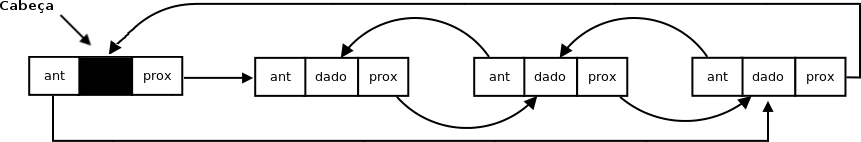
\includegraphics[width=300pt]{imgs/lista_circular.png}
  \label{lista_circular}
\end{figure}
\end{frame}

%------------------------------------------------

\begin{frame}
\frametitle{Lista Circular - Implementação}
% \scalebox{0.5}{
\begin{algorithm}[H]
\caption{ListaCircularBuscar} 
\label{ListaBuscar}
\Entrada{Lista C, item $x$.}
\Saida{Nó da lista que contém o item $x$ ou NULL caso não encontrado.}
\Inicio{
  aux $\leftarrow$ C.cabeça.prox \\
  \Enqto {(aux $\neq$ C.cabeça) AND (aux.item $\neq$ x) } {
      aux $\leftarrow$ aux.prox \\
  }
  \Retorna aux
}
\end{algorithm}
% }  
\end{frame}

%------------------------------------------------

\begin{frame}
\frametitle{Lista Circular - Implementação}
% \scalebox{0.5}{
\begin{algorithm}[H]
\caption{ListaCircularInserir} 
\label{ListaCircularInserir}
\Entrada{Lista circular $C$, item $x$.}
\Inicio{
  novo $\leftarrow$ ALOCA\_NODO()\\
  novo.item $\leftarrow$ x \\
  novo.prox $\leftarrow$ C.cabeça.prox \\
  C.cabeça.prox.ant $\leftarrow$ novo \\
  C.cabeça.prox $\leftarrow$ novo \\
  novo.ant $\leftarrow$ C.cabeça \\
}
\end{algorithm}
% }  
\end{frame}


%------------------------------------------------

\begin{frame}
\frametitle{Lista Circular - Implementação}
\scalebox{0.9}{
\begin{algorithm}[H]
\caption{ListaCircularRemover} 
\label{ListaCircularRemover}
\Entrada{Lista C, item $x$.}
\Saida{V ou F.}
\Inicio{
    aux $\leftarrow$ ListaCircularBuscar(C, $x$) \\
    \Se {(aux $\neq$ C.cabeça)} {
      aux.ant.prox $\leftarrow$ aux.prox \\
      aux.prox.ant $\leftarrow$ aux.ant \\
      aux.prox $\leftarrow$ NULL\\
      aux.ant $\leftarrow$ NULL\\    
      DESALOCA\_NODO(aux) \\
      \Retorna Verdadeiro
    }
    \Senao {
      \Retorna Falso
    }
}
\end{algorithm}
}  
\end{frame}

%------------------------------------------------
%
%\begin{frame}
%\frametitle{Exercício}
%
%Escrever em pseudo-código as operações básicas em pilha e fila utilizando listas duplamente encadeadas.
%
%\end{frame}
%

%------------------------------------------------
\section{Conclusão}
%------------------------------------------------
\begin{frame}
\frametitle{Conclusão}

\begin{block} {Material de apoio}
 Animações das operações disponíveis em \href{https://www.ime.usp.br/~nelio/ensino/2002-1/ed/}{http://www.ime.usp.br/\~{ }nelio/ensino/2002-1/ed/}
\end{block}
\begin{block}{Livro Base}
Projeto de Algoritmos - Nívio Ziviani - Capítulo 3, Seção 3.2 e 3.3
\end{block}
%\begin{block} {Próxima aula}
% Árvores
%\end{block}
\end{frame}


%------------------------------------------------

\begin{frame}
\titlepage % Print the title page as the first slide

\begin{figure}[!h]
  \centering
   
\includegraphics[width=80pt]{imgs/introducao.png}
  \label{fig_introducao}
\end{figure}
\end{frame}

%----------------------------------------------------------------------------------------


\end{document} 